\chapter{几何}

\index{几何}

在几何问题中，找到一种合适的方法来处理问题往往具有挑战性，
需要使得问题的解决方案能够方便地实现，并且特殊情况的数量较少。

作为一个例子，考虑这样一个问题：
给定一个四边形的顶点
（有四个顶点的多边形），
我们的任务是计算它的面积。
例如，该问题的一个可能的输入如下：

\begin{center}
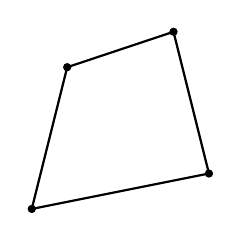
\begin{tikzpicture}[scale=0.45]

\draw[fill] (6,2) circle [radius=0.1];
\draw[fill] (5,6) circle [radius=0.1];
\draw[fill] (2,5) circle [radius=0.1];
\draw[fill] (1,1) circle [radius=0.1];
\draw[thick] (6,2) -- (5,6) -- (2,5) -- (1,1) -- (6,2);
\end{tikzpicture}
\end{center}
解决这个问题的一种方法是通过两个对角顶点之间的直线
将四边形分成两个三角形：
\begin{center}
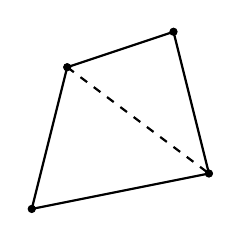
\begin{tikzpicture}[scale=0.45]

\draw[fill] (6,2) circle [radius=0.1];
\draw[fill] (5,6) circle [radius=0.1];
\draw[fill] (2,5) circle [radius=0.1];
\draw[fill] (1,1) circle [radius=0.1];

\draw[thick] (6,2) -- (5,6) -- (2,5) -- (1,1) -- (6,2);
\draw[dashed,thick] (2,5) -- (6,2);
\end{tikzpicture}
\end{center}
然后，只需将两个三角形的面积相加即可。
三角形的面积可以通过例如\key{海伦公式}计算
%\footnote{Heron of Alexandria (c. 10--70) was a Greek mathematician.}
\[ \sqrt{s (s-a) (s-b) (s-c)},\]
其中 $a$、$b$ 和 $c$ 是
三角形各边的长度，
$s=(a+b+c)/2$。
\index{海伦公式}

这是解决问题的一种可能方法，
但有一个陷阱：
如何将四边形分成三角形？
事实证明，有时我们不能简单地选取
两个任意的对角顶点。
例如，在以下情况中，
分割线在四边形的\emph{外部}：
\begin{center}
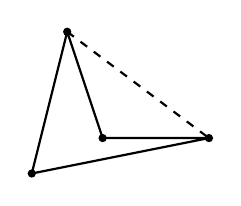
\begin{tikzpicture}[scale=0.45]

\draw[fill] (6,2) circle [radius=0.1];
\draw[fill] (3,2) circle [radius=0.1];
\draw[fill] (2,5) circle [radius=0.1];
\draw[fill] (1,1) circle [radius=0.1];
\draw[thick] (6,2) -- (3,2) -- (2,5) -- (1,1) -- (6,2);

\draw[dashed,thick] (2,5) -- (6,2);
\end{tikzpicture}
\end{center}
然而，用另一种方式画线就可以了：
\begin{center}
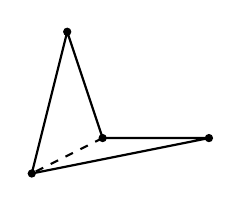
\begin{tikzpicture}[scale=0.45]

\draw[fill] (6,2) circle [radius=0.1];
\draw[fill] (3,2) circle [radius=0.1];
\draw[fill] (2,5) circle [radius=0.1];
\draw[fill] (1,1) circle [radius=0.1];
\draw[thick] (6,2) -- (3,2) -- (2,5) -- (1,1) -- (6,2);

\draw[dashed,thick] (3,2) -- (1,1);
\end{tikzpicture}
\end{center}
对于人类来说，哪条线是正确的选择是很明显的，
但对于计算机来说情况却很困难。
                           
然而，事实证明我们可以用
另一种更适合程序员的方法来解决这个问题。
即，有一个通用公式
\[x_1y_2-x_2y_1+x_2y_3-x_3y_2+x_3y_4-x_4y_3+x_4y_1-x_1y_4,\]
可以计算顶点为
$(x_1,y_1)$、
$(x_2,y_2)$、
$(x_3,y_3)$ 和
$(x_4,y_4)$ 的四边形的面积。
这个公式很容易实现，没有特殊情况，
我们甚至可以将该公式推广到\emph{所有}多边形。

\section{复数}

\index{复数}
\index{点}
\index{向量}

\key{复数}是形如 $x+y i$ 的数，
其中 $i = \sqrt{-1}$ 是\key{虚数单位}。
复数的几何解释是
它表示二维点 $(x,y)$
或从原点到点 $(x,y)$ 的向量。

例如，$4+2i$ 对应于以下
点和向量：

\begin{center}
\begin{tikzpicture}[scale=0.45]

\draw[->,thick] (-5,0)--(5,0);
\draw[->,thick] (0,-5)--(0,5);

\draw[fill] (4,2) circle [radius=0.1];
\draw[->,thick] (0,0)--(4-0.1,2-0.1);

\node at (4,2.8) {$(4,2)$};
\end{tikzpicture}
\end{center}

\index{complex@\texttt{complex}}

C++ 的复数类 \texttt{complex} 在
解决几何问题时非常有用。
使用这个类，我们可以将点和向量
表示为复数，并且该类包含
在几何中有用的工具。

在以下代码中，\texttt{C} 是坐标的类型，
\texttt{P} 是点或向量的类型。
此外，代码定义了宏 \texttt{X} 和 \texttt{Y}，
可用于引用 x 和 y 坐标。

\begin{lstlisting}
typedef long long C;
typedef complex<C> P;
#define X real()
#define Y imag()
\end{lstlisting}

例如，以下代码定义了一个点 $p=(4,2)$
并打印其 x 和 y 坐标：

\begin{lstlisting}
P p = {4,2};
cout << p.X << " " << p.Y << "\n"; // 4 2
\end{lstlisting}

以下代码定义了向量 $v=(3,1)$ 和 $u=(2,2)$，
然后计算它们的和 $s=v+u$。

\begin{lstlisting}
P v = {3,1};
P u = {2,2};
P s = v+u;
cout << s.X << " " << s.Y << "\n"; // 5 3
\end{lstlisting}

在实践中，合适的坐标类型通常是
\texttt{long long}（整数）或 \texttt{long double}
（实数）。
尽可能使用整数是个好主意，
因为整数的运算是精确的。
如果需要使用实数，
在比较数字时应考虑精度误差。
检查实数 $a$ 和 $b$ 是否相等的安全方法
是使用 $|a-b|<\epsilon$ 进行比较，
其中 $\epsilon$ 是一个很小的数（例如 $\epsilon=10^{-9}$）。

\subsubsection*{函数}

在以下示例中，坐标类型为
\texttt{long double}。

函数 $\texttt{abs}(v)$ 使用公式
$\sqrt{x^2+y^2}$ 计算向量 $v=(x,y)$
的长度 $|v|$。
该函数也可用于
计算点
$(x_1,y_1)$ 和 $(x_2,y_2)$ 之间的距离，
因为该距离等于
向量 $(x_2-x_1,y_2-y_1)$ 的长度。

以下代码计算点
$(4,2)$ 和 $(3,-1)$ 之间的距离：
\begin{lstlisting}
P a = {4,2};
P b = {3,-1};
cout << abs(b-a) << "\n"; // 3.16228
\end{lstlisting}

函数 $\texttt{arg}(v)$ 计算向量
$v=(x,y)$ 相对于 x 轴的角度。
该函数返回的角度以弧度为单位，
其中 $r$ 弧度等于 $180 r/\pi$ 度。
向右指的向量的角度为 0，
角度顺时针递减，逆时针递增。

函数 $\texttt{polar}(s,a)$ 构造一个
长度为 $s$ 且指向角度 $a$ 的向量。
通过将一个向量乘以长度为 1、角度为 $a$ 的向量，
可以将该向量旋转角度 $a$。

以下代码计算
向量 $(4,2)$ 的角度，
将其逆时针旋转 $1/2$ 弧度，
然后再次计算角度：

\begin{lstlisting}
P v = {4,2};
cout << arg(v) << "\n"; // 0.463648
v *= polar(1.0,0.5);
cout << arg(v) << "\n"; // 0.963648
\end{lstlisting}

\section{点与直线}

\index{叉积}

向量 $a=(x_1,y_1)$ 和 $b=(x_2,y_2)$ 的\key{叉积}
$a \times b$ 使用公式 $x_1 y_2 - x_2 y_1$ 计算。
叉积告诉我们当 $b$ 直接接在 $a$ 之后时，
$b$ 是向左转（正值）、不转弯（零）
还是向右转（负值）。

下图说明了上述情况：
\begin{center}
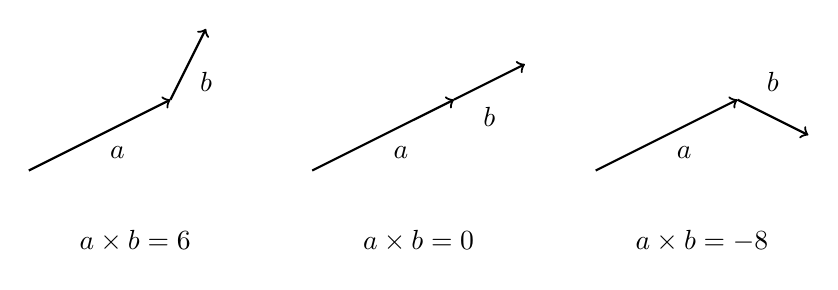
\begin{tikzpicture}[scale=0.45]

\draw[->,thick] (0,0)--(4,2);
\draw[->,thick] (4,2)--(4+1,2+2);

\node at (2.5,0.5) {$a$};
\node at (5,2.5) {$b$};

\node at (3,-2) {$a \times b = 6$};

\draw[->,thick] (8+0,0)--(8+4,2);
\draw[->,thick] (8+4,2)--(8+4+2,2+1);

\node at (8+2.5,0.5) {$a$};
\node at (8+5,1.5) {$b$};

\node at (8+3,-2) {$a \times b = 0$};

\draw[->,thick] (16+0,0)--(16+4,2);
\draw[->,thick] (16+4,2)--(16+4+2,2-1);

\node at (16+2.5,0.5) {$a$};
\node at (16+5,2.5) {$b$};

\node at (16+3,-2) {$a \times b = -8$};
\end{tikzpicture}
\end{center}

\noindent
例如，在第一种情况中
$a=(4,2)$ 且 $b=(1,2)$。
以下代码使用 \texttt{complex} 类计算叉积：

\begin{lstlisting}
P a = {4,2};
P b = {1,2};
C p = (conj(a)*b).Y; // 6
\end{lstlisting}

上面的代码有效，因为
函数 \texttt{conj} 会取向量 y 坐标的相反数，
当向量 $(x_1,-y_1)$ 和 $(x_2,y_2)$
相乘时，结果的 y 坐标
为 $x_1 y_2 - x_2 y_1$。

\subsubsection{点的位置}

叉积可用于测试一个点位于直线的左侧还是右侧。
假设直线经过点 $s_1$ 和 $s_2$，
我们从 $s_1$ 向 $s_2$ 看，点为 $p$。

例如，在下图中，
$p$ 在直线的左侧：
\begin{center}
\begin{tikzpicture}[scale=0.45]
\draw[dashed,thick,->] (0,-3)--(12,6);
\draw[fill] (4,0) circle [radius=0.1];
\draw[fill] (8,3) circle [radius=0.1];
\draw[fill] (5,3) circle [radius=0.1];
\node at (4,-1) {$s_1$};
\node at (8,2) {$s_2$};
\node at (5,4) {$p$};
\end{tikzpicture}
\end{center}

叉积 $(p-s_1) \times (p-s_2)$
告诉我们点 $p$ 的位置。
如果叉积为正，
则 $p$ 位于左侧；
如果叉积为负，
则 $p$ 位于右侧。
最后，如果叉积为零，
则点 $s_1$、$s_2$ 和 $p$ 在同一条直线上。

\subsubsection{线段相交}

\index{线段相交}

接下来我们考虑测试两条线段
$ab$ 和 $cd$ 是否相交的问题。可能的情况有：

\textit{情况 1：}
两条线段在同一条直线上
并且互相重叠。
在这种情况下，交点有无限多个。
例如，在下图中，
$c$ 和 $b$ 之间的所有点都是
交点：
\begin{center}
\begin{tikzpicture}[scale=0.9]
\draw (1.5,1.5)--(6,3);
\draw (0,1)--(4.5,2.5);
\draw[fill] (0,1) circle [radius=0.05];
\node at (0,0.5) {$a$};
\draw[fill] (1.5,1.5) circle [radius=0.05];
\node at (6,2.5) {$d$};
\draw[fill] (4.5,2.5) circle [radius=0.05];
\node at (1.5,1) {$c$};
\draw[fill] (6,3) circle [radius=0.05];
\node at (4.5,2) {$b$};
\end{tikzpicture}
\end{center}

在这种情况下，我们可以使用叉积来
检查所有点是否在同一条直线上。
然后，我们可以对点进行排序并
检查两条线段是否互相重叠。

\textit{情况 2：}
两条线段有一个公共顶点，
且该顶点是唯一的交点。
例如，在下图中，
交点为 $b=c$：

\begin{center}
\begin{tikzpicture}[scale=0.9]
\draw (0,0)--(4,2);
\draw (4,2)--(6,1);
\draw[fill] (0,0) circle [radius=0.05];
\draw[fill] (4,2) circle [radius=0.05];
\draw[fill] (6,1) circle [radius=0.05];

\node at (0,0.5) {$a$};
\node at (4,2.5) {$b=c$};
\node at (6,1.5) {$d$};
\end{tikzpicture}
\end{center}

这种情况很容易检查，因为
交点只有四种可能：
$a=c$、$a=d$、$b=c$ 和 $b=d$。

\textit{情况 3：}
恰好有一个交点，
且该交点不是任何线段的顶点。
在下图中，点 $p$
是交点：
\begin{center}
\begin{tikzpicture}[scale=0.9]
\draw (0,1)--(6,3);
\draw (2,4)--(4,0);
\draw[fill] (0,1) circle [radius=0.05];
\node at (0,0.5) {$c$};
\draw[fill] (6,3) circle [radius=0.05];
\node at (6,2.5) {$d$};
\draw[fill] (2,4) circle [radius=0.05];
\node at (1.5,3.5) {$a$};
\draw[fill] (4,0) circle [radius=0.05];
\node at (4,-0.4) {$b$};
\draw[fill] (3,2) circle [radius=0.05];
\node at (3,1.5) {$p$};
\end{tikzpicture}
\end{center}

在这种情况下，当点 $c$ 和 $d$ 分别在
经过 $a$ 和 $b$ 的直线的不同侧，
且点 $a$ 和 $b$ 分别在
经过 $c$ 和 $d$ 的直线的不同侧时，
两条线段恰好相交。
我们可以使用叉积来检查这一点。

\subsubsection{点到直线的距离}

叉积的另一个特性是可以
使用公式
\[\frac{| (a-c) \times (b-c) |}{2},\]
计算三角形的面积，
其中 $a$、$b$ 和 $c$ 是三角形的顶点。
利用这一事实，我们可以推导出
计算点与直线之间最短距离的公式。
例如，在下图中 $d$ 是
点 $p$ 与由点 $s_1$ 和 $s_2$ 定义的直线之间的
最短距离：
\begin{center}
\begin{tikzpicture}[scale=0.75]
\draw (-2,-1)--(6,3);
\draw[dashed] (1,4)--(2.40,1.2);
\node at (0,-0.5) {$s_1$};
\node at (4,1.5) {$s_2$};
\node at (0.5,4) {$p$};
\node at (2,2.7) {$d$};
\draw[fill] (0,0) circle [radius=0.05];
\draw[fill] (4,2) circle [radius=0.05];
\draw[fill] (1,4) circle [radius=0.05];
\end{tikzpicture}
\end{center}

顶点为 $s_1$、$s_2$ 和 $p$ 的三角形的面积
可以用两种方式计算：
它既等于
$\frac{1}{2} |s_2-s_1| d$，
也等于
$\frac{1}{2} ((s_1-p) \times (s_2-p))$。
因此，最短距离为
\[ d = \frac{(s_1-p) \times (s_2-p)}{|s_2-s_1|} .\]

\subsubsection{点在多边形内部}

现在我们来考虑测试一个点
位于多边形内部还是外部的问题。
例如，在下图中点 $a$
在多边形内部，点 $b$ 在多边形外部。

\begin{center}
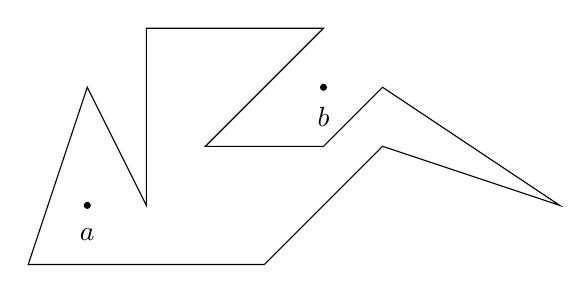
\begin{tikzpicture}[scale=0.75]
%\draw (0,0)--(2,-2)--(3,1)--(5,1)--(2,3)--(1,2)--(-1,2)--(1,4)--(-2,4)--(-2,1)--(-3,3)--(-4,0)--(0,0);
\draw (0,0)--(2,2)--(5,1)--(2,3)--(1,2)--(-1,2)--(1,4)--(-2,4)--(-2,1)--(-3,3)--(-4,0)--(0,0);

\draw[fill] (-3,1) circle [radius=0.05];
\node at (-3,0.5) {$a$};
\draw[fill] (1,3) circle [radius=0.05];
\node at (1,2.5) {$b$};
\end{tikzpicture}
\end{center}

解决这个问题的一种方便方法是从该点
向任意方向发射一条\emph{射线}，
并计算它与多边形边界相交的次数。
如果次数为奇数，
则点在多边形内部，
如果次数为偶数，
则点在多边形外部。

\begin{samepage}
例如，我们可以发射以下射线：
\begin{center}
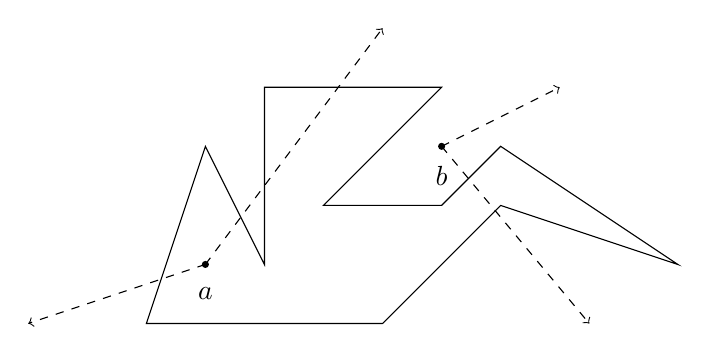
\begin{tikzpicture}[scale=0.75]
\draw (0,0)--(2,2)--(5,1)--(2,3)--(1,2)--(-1,2)--(1,4)--(-2,4)--(-2,1)--(-3,3)--(-4,0)--(0,0);

\draw[fill] (-3,1) circle [radius=0.05];
\node at (-3,0.5) {$a$};
\draw[fill] (1,3) circle [radius=0.05];
\node at (1,2.5) {$b$};

\draw[dashed,->] (-3,1)--(-6,0);
\draw[dashed,->] (-3,1)--(0,5);

\draw[dashed,->] (1,3)--(3.5,0);
\draw[dashed,->] (1,3)--(3,4);
\end{tikzpicture}
\end{center}
\end{samepage}

从 $a$ 发出的射线分别与多边形边界
相交 1 次和 3 次，
所以 $a$ 在多边形内部。
相应地，从 $b$ 发出的射线
分别与多边形边界相交 0 次和 2 次，
所以 $b$ 在多边形外部。

\section{多边形面积}

计算多边形面积的通用公式，
有时称为\key{鞋带公式}，
如下所示：\index{鞋带公式}
\[\frac{1}{2} |\sum_{i=1}^{n-1} (p_i \times p_{i+1})| =
\frac{1}{2} |\sum_{i=1}^{n-1} (x_i y_{i+1} - x_{i+1} y_i)|, \]
这里顶点为
$p_1=(x_1,y_1)$、$p_2=(x_2,y_2)$、$\ldots$、$p_n=(x_n,y_n)$，
其顺序满足
$p_i$ 和 $p_{i+1}$ 是多边形边界上相邻的顶点，
且第一个和最后一个顶点相同，即 $p_1=p_n$。

例如，以下多边形的面积
\begin{center}
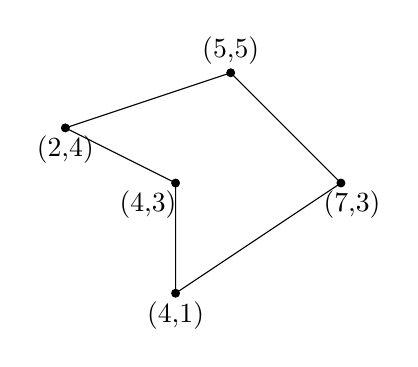
\begin{tikzpicture}[scale=0.7]
\filldraw (4,1.4) circle (2pt);
\filldraw (7,3.4) circle (2pt);
\filldraw (5,5.4) circle (2pt);
\filldraw (2,4.4) circle (2pt);
\filldraw (4,3.4) circle (2pt);
\node (1) at (4,1) {(4,1)};
\node (2) at (7.2,3) {(7,3)};
\node (3) at (5,5.8) {(5,5)};
\node (4) at (2,4) {(2,4)};
\node (5) at (3.5,3) {(4,3)};
\path[draw] (4,1.4) -- (7,3.4) -- (5,5.4) -- (2,4.4) -- (4,3.4) -- (4,1.4);
\end{tikzpicture}
\end{center}
为
\[\frac{|(2\cdot5-5\cdot4)+(5\cdot3-7\cdot5)+(7\cdot1-4\cdot3)+(4\cdot3-4\cdot1)+(4\cdot4-2\cdot3)|}{2} = 17/2.\]

该公式的思想是遍历梯形，
这些梯形的一边是多边形的一条边，
另一边位于水平线 $y=0$ 上。
例如：
\begin{center}
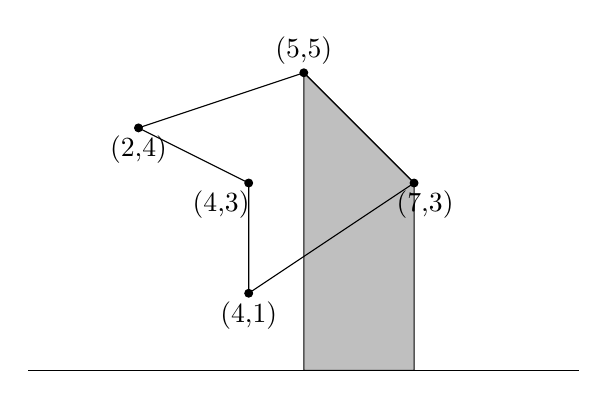
\begin{tikzpicture}[scale=0.7]
\path[draw,fill=lightgray] (5,5.4) -- (7,3.4) -- (7,0) -- (5,0) -- (5,5.4);
\filldraw (4,1.4) circle (2pt);
\filldraw (7,3.4) circle (2pt);
\filldraw (5,5.4) circle (2pt);
\filldraw (2,4.4) circle (2pt);
\filldraw (4,3.4) circle (2pt);
\node (1) at (4,1) {(4,1)};
\node (2) at (7.2,3) {(7,3)};
\node (3) at (5,5.8) {(5,5)};
\node (4) at (2,4) {(2,4)};
\node (5) at (3.5,3) {(4,3)};
\path[draw] (4,1.4) -- (7,3.4) -- (5,5.4) -- (2,4.4) -- (4,3.4) -- (4,1.4);
\draw (0,0) -- (10,0);
\end{tikzpicture}
\end{center}
这样一个梯形的面积为
\[(x_{i+1}-x_{i}) \frac{y_i+y_{i+1}}{2},\]
其中多边形的顶点为 $p_i$ 和 $p_{i+1}$。
如果 $x_{i+1}>x_{i}$，则面积为正，
如果 $x_{i+1}<x_{i}$，则面积为负。

多边形的面积是所有这些梯形面积的总和，
由此得到公式
\[|\sum_{i=1}^{n-1} (x_{i+1}-x_{i}) \frac{y_i+y_{i+1}}{2}| =
\frac{1}{2} |\sum_{i=1}^{n-1} (x_i y_{i+1} - x_{i+1} y_i)|.\]

注意这里取的是和的绝对值，
因为和的值可能是正的也可能是负的，
取决于我们是顺时针还是逆时针
沿着多边形的边界行走。

\subsubsection{Pick定理}

\index{Pick定理}

\key{Pick定理}提供了另一种计算
多边形面积的方法，条件是多边形
的所有顶点都具有整数坐标。
根据Pick定理，多边形的面积为
\[ a + b/2 -1,\]
其中 $a$ 是多边形内部的整数点数，
$b$ 是多边形边界上的整数点数。

例如，以下多边形的面积
\begin{center}
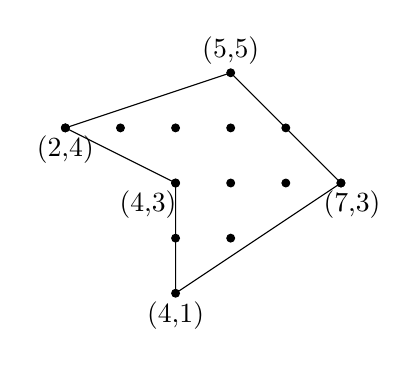
\begin{tikzpicture}[scale=0.7]
\filldraw (4,1.4) circle (2pt);
\filldraw (7,3.4) circle (2pt);
\filldraw (5,5.4) circle (2pt);
\filldraw (2,4.4) circle (2pt);
\filldraw (4,3.4) circle (2pt);
\node (1) at (4,1) {(4,1)};
\node (2) at (7.2,3) {(7,3)};
\node (3) at (5,5.8) {(5,5)};
\node (4) at (2,4) {(2,4)};
\node (5) at (3.5,3) {(4,3)};
\path[draw] (4,1.4) -- (7,3.4) -- (5,5.4) -- (2,4.4) -- (4,3.4) -- (4,1.4);

\filldraw (2,4.4) circle (2pt);
\filldraw (3,4.4) circle (2pt);
\filldraw (4,4.4) circle (2pt);
\filldraw (5,4.4) circle (2pt);
\filldraw (6,4.4) circle (2pt);

\filldraw (4,3.4) circle (2pt);
\filldraw (5,3.4) circle (2pt);
\filldraw (6,3.4) circle (2pt);
\filldraw (7,3.4) circle (2pt);

\filldraw (4,2.4) circle (2pt);
\filldraw (5,2.4) circle (2pt);
\end{tikzpicture}
\end{center}
为 $6+7/2-1=17/2$。

\section{距离函数}

\index{距离函数}
\index{欧几里得距离}
\index{曼哈顿距离}

\key{距离函数}定义两个点之间的距离。
通常的距离函数是
\key{欧几里得距离}，其中点
$(x_1,y_1)$ 和 $(x_2,y_2)$ 之间的距离为
\[\sqrt{(x_2-x_1)^2+(y_2-y_1)^2}.\]
另一种距离函数是
\key{曼哈顿距离}，
其中点
$(x_1,y_1)$ 和 $(x_2,y_2)$ 之间的距离为
\[|x_1-x_2|+|y_1-y_2|.\]
\begin{samepage}
例如，考虑下图：
\begin{center}
\begin{tikzpicture}

\draw[fill] (2,1) circle [radius=0.05];
\draw[fill] (5,2) circle [radius=0.05];

\node at (2,0.5) {$(2,1)$};
\node at (5,1.5) {$(5,2)$};

\draw[dashed] (2,1) -- (5,2);

\draw[fill] (5+2,1) circle [radius=0.05];
\draw[fill] (5+5,2) circle [radius=0.05];

\node at (5+2,0.5) {$(2,1)$};
\node at (5+5,1.5) {$(5,2)$};

\draw[dashed] (5+2,1) -- (5+2,2);
\draw[dashed] (5+2,2) -- (5+5,2);

\node at (3.5,-0.5) {欧几里得距离};
\node at (5+3.5,-0.5) {曼哈顿距离};
\end{tikzpicture}
\end{center}
\end{samepage}
两点之间的欧几里得距离为
\[\sqrt{(5-2)^2+(2-1)^2}=\sqrt{10}\]
曼哈顿距离为
\[|5-2|+|2-1|=4.\]
下图显示了在欧几里得距离和曼哈顿距离下，
距离中心点 1 以内的区域：
\begin{center}
\begin{tikzpicture}

\draw[fill=gray!20] (0,0) circle [radius=1];
\draw[fill] (0,0) circle [radius=0.05];

\node at (0,-1.5) {欧几里得距离};

\draw[fill=gray!20] (5+0,1) -- (5-1,0) -- (5+0,-1) -- (5+1,0) -- (5+0,1);
\draw[fill] (5,0) circle [radius=0.05];
\node at (5,-1.5) {曼哈顿距离};
\end{tikzpicture}
\end{center}

\subsubsection{坐标旋转}

如果使用曼哈顿距离而不是欧几里得距离，
某些问题会更容易解决。
作为一个例子，考虑这样一个问题：给定二维平面上
$n$ 个点，
我们的任务是计算任意两点之间的最大曼哈顿距离。

例如，考虑以下点集：
\begin{center}
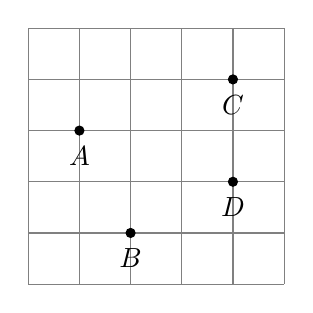
\begin{tikzpicture}[scale=0.65]
\draw[color=gray] (-1,-1) grid (4,4);

\filldraw (0,2) circle (2.5pt);
\filldraw (3,3) circle (2.5pt);
\filldraw (1,0) circle (2.5pt);
\filldraw (3,1) circle (2.5pt);

\node at (0,1.5) {$A$};
\node at (3,2.5) {$C$};
\node at (1,-0.5) {$B$};
\node at (3,0.5) {$D$};
\end{tikzpicture}
\end{center}
点 $B$ 和 $C$ 之间的最大曼哈顿距离为 5：
\begin{center}
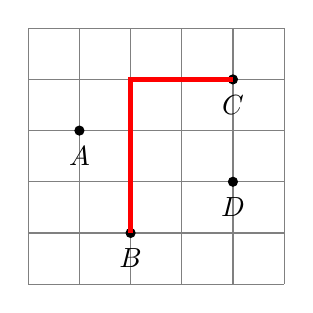
\begin{tikzpicture}[scale=0.65]
\draw[color=gray] (-1,-1) grid (4,4);

\filldraw (0,2) circle (2.5pt);
\filldraw (3,3) circle (2.5pt);
\filldraw (1,0) circle (2.5pt);
\filldraw (3,1) circle (2.5pt);

\node at (0,1.5) {$A$};
\node at (3,2.5) {$C$};
\node at (1,-0.5) {$B$};
\node at (3,0.5) {$D$};

\path[draw=red,thick,line width=2pt] (1,0) -- (1,3) -- (3,3);
\end{tikzpicture}
\end{center}

与曼哈顿距离相关的一个有用技巧是
将所有坐标旋转 45 度，
使得点 $(x,y)$ 变为 $(x+y,y-x)$。
例如，旋转上述点后，
结果为：

\begin{center}
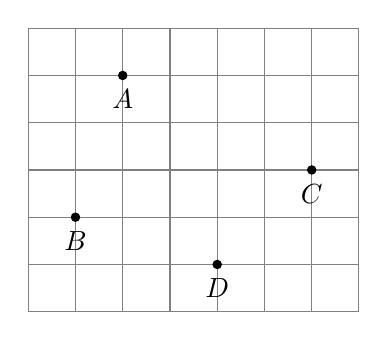
\begin{tikzpicture}[scale=0.6]
\draw[color=gray] (0,-3) grid (7,3);

\filldraw (2,2) circle (2.5pt);
\filldraw (6,0) circle (2.5pt);
\filldraw (1,-1) circle (2.5pt);
\filldraw (4,-2) circle (2.5pt);

\node at (2,1.5) {$A$};
\node at (6,-0.5) {$C$};
\node at (1,-1.5) {$B$};
\node at (4,-2.5) {$D$};
\end{tikzpicture}
\end{center}
最大距离如下：
\begin{center}
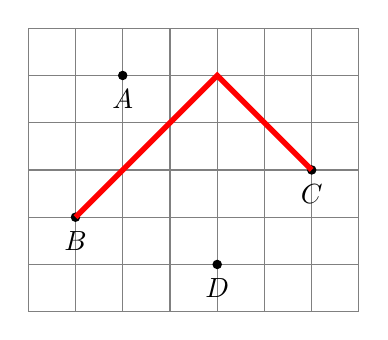
\begin{tikzpicture}[scale=0.6]
\draw[color=gray] (0,-3) grid (7,3);

\filldraw (2,2) circle (2.5pt);
\filldraw (6,0) circle (2.5pt);
\filldraw (1,-1) circle (2.5pt);
\filldraw (4,-2) circle (2.5pt);

\node at (2,1.5) {$A$};
\node at (6,-0.5) {$C$};
\node at (1,-1.5) {$B$};
\node at (4,-2.5) {$D$};

\path[draw=red,thick,line width=2pt] (1,-1) -- (4,2) -- (6,0);
\end{tikzpicture}
\end{center}

考虑两个点 $p_1=(x_1,y_1)$ 和 $p_2=(x_2,y_2)$，其旋转后
的坐标为 $p'_1=(x'_1,y'_1)$ 和 $p'_2=(x'_2,y'_2)$。
现在有两种方式来表示
$p_1$ 和 $p_2$ 之间的曼哈顿距离：
\[|x_1-x_2|+|y_1-y_2| = \max(|x'_1-x'_2|,|y'_1-y'_2|)\]

例如，如果 $p_1=(1,0)$ 且 $p_2=(3,3)$，
旋转后的坐标为 $p'_1=(1,-1)$ 和 $p'_2=(6,0)$，
曼哈顿距离为
\[|1-3|+|0-3| = \max(|1-6|,|-1-0|) = 5.\]

旋转后的坐标提供了一种简单的
处理曼哈顿距离的方法，因为我们可以
分别考虑 x 和 y 坐标。
要最大化两点之间的曼哈顿距离，
我们应该找到旋转后的坐标能使以下值最大化的
两个点：
\[\max(|x'_1-x'_2|,|y'_1-y'_2|).\]
这很简单，因为旋转后坐标的
水平或垂直差值中必有一个是最大的。
